%************************************************
\chapter{Preliminaries}\label{ch:prelim}
%************************************************

The goal of this chapter is to provide a formal background on the covered material, together with a unified notation (which differs quite a lot from publication to publication). After we establish some basic theoretical foundations in \secref{prelim:essentials}, we remind the reader of the basic notions of reinforcement learning in \secref{prelim:rl} and of the recently explored and useful distributional reinforcement learning in \secref{prelim:distrl}. We follow up with the basics of risk together with the crucial CVaR measure in \secref{prelim:risk}.

The interested reader is welcome to explore the books and publications referenced throughout this chapter and in \secref{prelim:literature}. An informed reader may choose to skip to \secref{prelim:problem} where we formalize the problems tackled in this thesis.


%***********************************************************************************************************************************************************
%***********************************************************************************************************************************************************
%***********************************************************************************************************************************************************


\section{Reinforcement Learning}\label{sec:prelim:rl}

The idea that we learn by interacting with our environment is probably the first to occur to us when we think about the nature of learning. Reinforcement learning \cite{sutton1998reinforcement} is a sub-field of machine learning that deals with time-dependent decision making in an unknown environment. The learner (often called agent) is not told which actions to take, but instead must discover which actions yield the most reward by trying them out. In the most interesting and challenging cases, actions may affect not only the immediate reward but also subsequent situations and rewards. These two characteristics, trial-and-error search and delayed reward are the most important distinguishing features of reinforcement learning.

The general interaction between the agent and an environment can be seen in \figref{rlloop}. In each time-step $t$, the agent receives an observation $x_t$ and a reward $r_t$ and picks an action $a_t$ and the process repeats. Below we formalize all the necessary notions of states, actions and rewards as a Markov Decision Process.

\begin{figure}[h]
\center
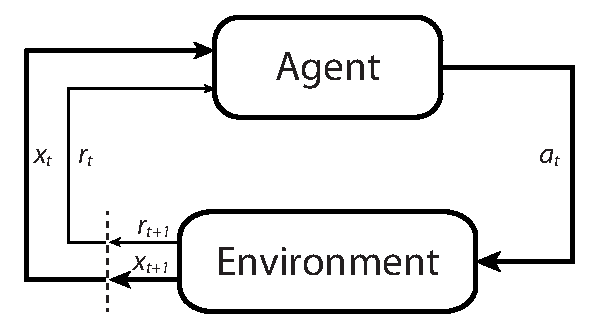
\includegraphics[width=.6\linewidth]{gfx/rl_loop.pdf}
\caption{The Reinforcement learning cycle}
\label{fig:rlloop}
\end{figure}

\subsection{Markov Decision Processes}

Markov Decision Process (MDP, \citet{bellman1957markovian}) is a classical formalization of sequential decision making, where actions influence not just immediate rewards, but also subsequent situations, or states, and through those future rewards. They are a mathematically idealized form of the reinforcement learning problem for which precise theoretical statements can be made.

The word Markov points to the fact that we assume that the state transitions of an MDP satisfy the memoryless property. This means that the conditional probability distribution of future states of the process depends only upon the present state and not the whole history of events that preceded it.

\begin{definition}

MDP is a 5-tuple $\mathcal{M} = (\cX, \cA, r, p, \gamma)$, where 

$\cX$ is the finite state space

$\cA$ is the finite action space

$r(x, a)$ is a bounded deterministic\footnote{All the presented results are extendable to the case with random reward and with reward being a function of the transition $R(x, a, a')$. In fact, we use $R(x, a, a')$ in all our experiments. We avoid these extension for the sake of cleaner notation.} reward generated by being in state $x$ and selecting action $a$

$p(\cdot|x, a)$ is the transition probability distribution

$\gamma \in [0, 1)$ is a discount factor
\end{definition}
We will denote $x$ or $x_t$ as the states visited in time $t$ and $x'$ or $x_{t+1}$ states visited in time $t+1$.

\begin{definition}
A stationary (or Markovian) policy is a mapping from states to actions $\pi:\cX \to \cA$.
\end{definition}

%When solving MDPs with the usual discounted expected value criterion, it is common to limit the policy space to stationary policies, where the decision to take an action depends only on the current state. Unfortunately, when one considers other more general criteria, it is necessary to consider the whole action-state history that led up to the last state. This fact leads to the definition of a history-dependent policies.

\subsection{Return}

The ultimate goal of any reinforcement learning agent is to maximize some notion of reward, which is captured by the return. The two most commonly considered types of returns are the sum of rewards, or the mathematically convenient expected discounted reward. In this thesis we focus on the latter.


We define the return $Z^\pi(x)$ as a random variable representing the discounted reward along a trajectory generated by the MDP by following policy $\pi$, starting at state $x$:
\begin{equation}\label{eqn:return}
\begin{split}
&Z^\pi(x)=\sum_{t=0}^\infty \gamma^tr(x_t,a_t)\\
&x_t \sim p(\cdot|x_{t-1}, a_{t-1}), a_t \sim \pi, x_0 = x
\end{split}
\end{equation}

As a useful notation, we denote $Z^\pi(x, a)$ as the random variable representing the discounted reward along a trajectory generated by first selecting action $a$ and then following policy $\pi$.
\begin{equation}
\begin{split}
&Z^\pi(x, a)=\sum_{t=0}^\infty \gamma^tr(x_t,a_t)\\
&x_t \sim p(\cdot|x_{t-1}, a_{t-1}), a_t \sim \pi, x_0 = x, a_0 = a
\end{split}
\end{equation}

We will sometimes omit the superscript $\pi$ when the policy is clear from the context or is unimportant.

\subsection{Bellman equations}

The \textit{value function} $V^\pi : \cX\to\real$ of policy $\pi$ describes the expected return received from state $x \in \cX$ and acting according to $\pi$:
\begin{equation}
\begin{split}
V^\pi(x) = \expval{ Z^\pi(x)} =& \expect\left[\sum_{t=0}^\infty \gamma^tr(x_t,a_t) \right]\\
&x_0 = x, a_t \sim \pi
\end{split}
\end{equation}
The \textit{action-value} function $Q^\pi : \cX\times\cA\to\real$ of policy $\pi$ describes the expected return from taking action $a \in \cA$ from state $x \in \cX$, then acting according to $\pi$:
\begin{equation}
\begin{split}
Q^\pi(x, a) = \expval{Z^\pi(x, a)} =& \expect\left[ \sum_{t=0}^\infty \gamma^tr(x_t,a_t) \right]\\
&x_0 = x, a_0 = a, a_t \sim \pi
\end{split}
\end{equation}
Fundamental to reinforcement learning is the use of Bellman's equation \citep{bellman1957markovian} to describe the value and action-value functions by a recursive relationship:
\begin{align}
&V^\pi(x) = r\left(x, \pi(x)\right) + \gamma \expect\limits_{p, \pi}[ V^\pi(x')]\\
&Q^\pi(x, a) = r(x, a) + \gamma \expect_{p, \pi}[ V^\pi(x')]
\end{align}
As stated before, we are typically interested in maximizing the expected return. The most common approach for doing so involves the optimality equation
\begin{equation}\label{eqn:q}
Q^*(x,a) = r(x,a) + \gamma \expect\nolimits_p \bsquare{\max_{a' \in \cA} Q^*(x', a')}
\end{equation}
This equation has a unique fixed point $Q^*$ -  the optimal value function, corresponding to the set of optimal policies $\Pi^*$ ($\pi^*$ is optimal if $\expect_{a \sim \pi^*} Q^*(x, a) = \max_a Q^*(x,a)$).
We view value functions as vectors in $\mathbb{R}^{\cX \times \cA}$, and the expected reward function as one such vector. In this context, the \emph{Bellman operator} $\cT^\pi$ and \emph{optimality operator} $\cT$ are
\begin{align}
\cT^\pi Q(x,a) &:= r(x, a) + \gamma \expect_{P, \pi} [Q(x',a')]\\
\cT Q(x,a) &:= r(x, a) + \gamma \expect_{P} \bsquare{\max_{a' \in \cA}Q(x', a')}\label{eqn:bellmanoptimalityoperator}
\end{align}
These operators are useful as they describe the expected behaviour of popular learning algorithms such as SARSA and Q-Learning \cite{sutton1998reinforcement}. In particular they are both contraction mappings (see below), and their repeated application to some initial $Q_0$ converges exponentially to $Q^\pi$ or $Q^*$, respectively \citep{bertsekas1995neuro}.

\subsection{Contraction}\label{sec:contraction}
An important concept used in convergence analysis of reinforcement learning algorithms is that of a contraction.
\begin{definition}
A \textbf{fixed point} of a mapping $T: S\to S$ of a set $S$ into itself is $s\in S$ which is mapped onto itself, that is $Ts=s$.

Let $S=(S,d)$ be a metric space ($d$ is a metric on $S$). A mapping $T$ is called a \textbf{contraction} on $S$ if there exists a positive real number $\gamma < 1$ such that for all $s, t \in S$ we have $d(Ts, Tt) \le \gamma d(s,t)$.
\end{definition}

\begin{theorem}[Banach Fixed Point Theorem, Contraction Theorem]
Consider a metric space $S=(S,d)$, where $S \neq \emptyset$. Suppose that $S$ is complete (every Cauchy sequence in $S$ converges) and let $T$ be a contraction on $S$. Then $T$ has precisely one fixed point.
\end{theorem}


The takeaway for reinforcement learning is, that if $\cT$ is a contraction, by recursively applying $V_{t+1}=\cT V_t$ (here the operator maps value function $V_t \in \real$ to a new $V_{t+1} \in \real$), we converge to the single fixed point of this operator. This is used in convergence proofs for various RL operators, usually in combination with the infinity norm.

See e.g. \citet{kreyszig1989introductory} for a complete treatment of all mentioned concepts.



%***********************************************************************************************************************************************************
%***********************************************************************************************************************************************************
%***********************************************************************************************************************************************************


\section{Distributional Reinforcement Learning}\label{sec:prelim:distrl}

In contrast to standard reinforcement learning, where we model the expected return, in distributional reinforcement learning we aim to model the full distribution of the return. This is advantageous in cases where we want to e.g. model parametric uncertainty or design risk-sensitive algorithms \citep{morimura2010nonparametric, morimura2012parametric}. \citet{bellemare2017distributional} also argue, that the distributional approach is beneficial even in the case when we optimize the expected value, as the distribution gives us more information which helps the now commonly used approximate algorithms (such as DQN \citep{mnih2015human}).

At the core of the distributional approach lies the recursive equation of the return distribution:
\begin{equation}
\begin{split}
&Z(x, a) \overset{D}{=} r(x, a) + \gamma Z(x', a')\\
&x' \sim p(\cdot|x, a), a \sim \pi, x_0 = x, a_0 = a
\end{split}
\end{equation}

where $\overset{D}{=}$ denotes that random variables on both sides of the equation share the same probability distribution.

In the \emph{policy evaluation} setting \citep{sutton1998reinforcement} we are interested in the value function $V^\pi$ associated with a given policy $\pi$. The analogue here is the value distribution $Z^\pi$. Note that $Z^\pi$ describes the intrinsic randomness of the agent's interactions with its environment, rather than some measure of uncertainty about the environment itself.
%

We define the transition operator $P^\pi : \mathcal{Z} \to \mathcal{Z}$
\begin{equation}\label{eqn:transitionop}
\begin{split}
&P^\pi Z(x, a) \overset{D}{=} Z(x', a')\\
&x' \sim p(\cdot|x, a), a' \sim \pi
\end{split}
\end{equation}
We define the distributional Bellman operator $\cT^\pi : \mathcal{Z} \to \mathcal{Z}$ as
\begin{equation}
\cT^\pi Z(x,a) \overset{D}{=} r(x,a) + \gamma P^\pi Z(x,a).
\end{equation}
Note that this is a distributional equation and the distributional bellman operator is therefore fundamentally different from the standard bellman operator.

\citet{bellemare2017distributional} have shown, that the distributional bellman operator $\cT^\pi$ is not a contraction in the commonly used KL divergence \cite{kullback1997information}, but is a contraction in the infinity Wasserstein metric which we describe bellow, as it will become useful as a tool for evaluating algorithms in the rest of the thesis. Another important fact is, that the bellman optimality operator $\cT : \mathcal{Z}\to\mathcal{Z}$
\begin{equation}
\cT Z = \cT^\pi Z \quad \text{for some } \pi \text{ in the set of greedy policies}
\end{equation}
is not a contraction in any metric. The distribution does not converge to a fixed point, but rather to a sequence of optimal (in terms of expected value) policies. We encourage the interested reader to explore these topics in the excellent papers by \citet{bellemare2017distributional} and \citet{dabney2017distributional}.

\subsection{The Wasserstein Metric}
\newcommand{\pnorm}[1]{\| #1 \|_p}

One of the tools for analysis of distributional approaches to reinforcement learning is the Wasserstein metric $d_p$ between cumulative distribution functions (see e.g. \citet{bickel1981some}). The metric has recently gained in popularity and was used e.g. in unsupervised learning \citep{arjovsky2017wasserstein,bellemare2017cramer}. Unlike the Kullback-Leibler divergence, which strictly measures change in probability, the Wasserstein metric reflects the underlying geometry between outcomes.

For $F$, $G$ two c.d.fs over the reals, it is defined as
\begin{equation*}
d_p(F, G) := \inf_{U, V} \pnorm{U - V},
\end{equation*}
where the infimum is taken over all pairs of random variables $(U, V)$ with respective cumulative distributions $F$ and $G$. The infimum is attained by the inverse c.d.f. transform of a random variable $\mathcal{U}$ uniformly distributed on $[0, 1]$:
\begin{equation*}
d_p(F, G) = \| F^{-1}(\mathcal{U}) - G^{-1}(\mathcal{U}) \|_p .
\end{equation*}
For $p < \infty$ this is more explicitly written as
\begin{equation}
d_p(F, G) = \left ( \int_0^1 \big | F^{-1}(u) - G^{-1}(u) \big |^p du \right )^{1/p} .
\end{equation}
meaning it is an integral over the difference in the quantile functions of the random variables. This will become important later, as the quantile function has a direct connection to the CVaR objective \eqnref{problem} explored in this thesis.


%***********************************************************************************************************************************************************
%***********************************************************************************************************************************************************
%***********************************************************************************************************************************************************


\section{Risk-Sensitivity}\label{sec:prelim:risk}

The standard reinforcement learning agent that maximizes the expected reward which we discussed in the previous chapter does not take risk into account. Indeed in a mathematical sense, the shape of the reward distribution is unimportant as wildly different distributions may have the same expectation. This unfortunately is not the case in the real world, where there exist catastrophic losses - an investment company may have a good strategy that yields profit in expectation, but if the strategy is too risky and the company's capital drops under zero this investment strategy is useless. This leads us to defining risk, which describes the potential of gaining or losing reward and is therefore more expressive than a simple expectation.

The finance literature differentiates between three risk-related types of behavior, namely \textit{risk-neutral}, \textit{risk-averse} and \textit{risk-seeking}. We offer the following example to illustrate the differences between mentioned behaviors: Imagine you are facing two options, either (a) you get \$1 or (b) you get \$5 with 90\% probability, but lose \$35 with 10\% probability. A risk-neutral agent wouldn't differentiate between the two choices, as the expected value of reward is the same. A risk-averse agent would prefer option (a), as there is a risk of high losses in option (b). Risk-seeking agent would pick (b). The difference between the risk-sensitive behaviors can be visualized as in \figref{risk}.

\begin{figure}
\center
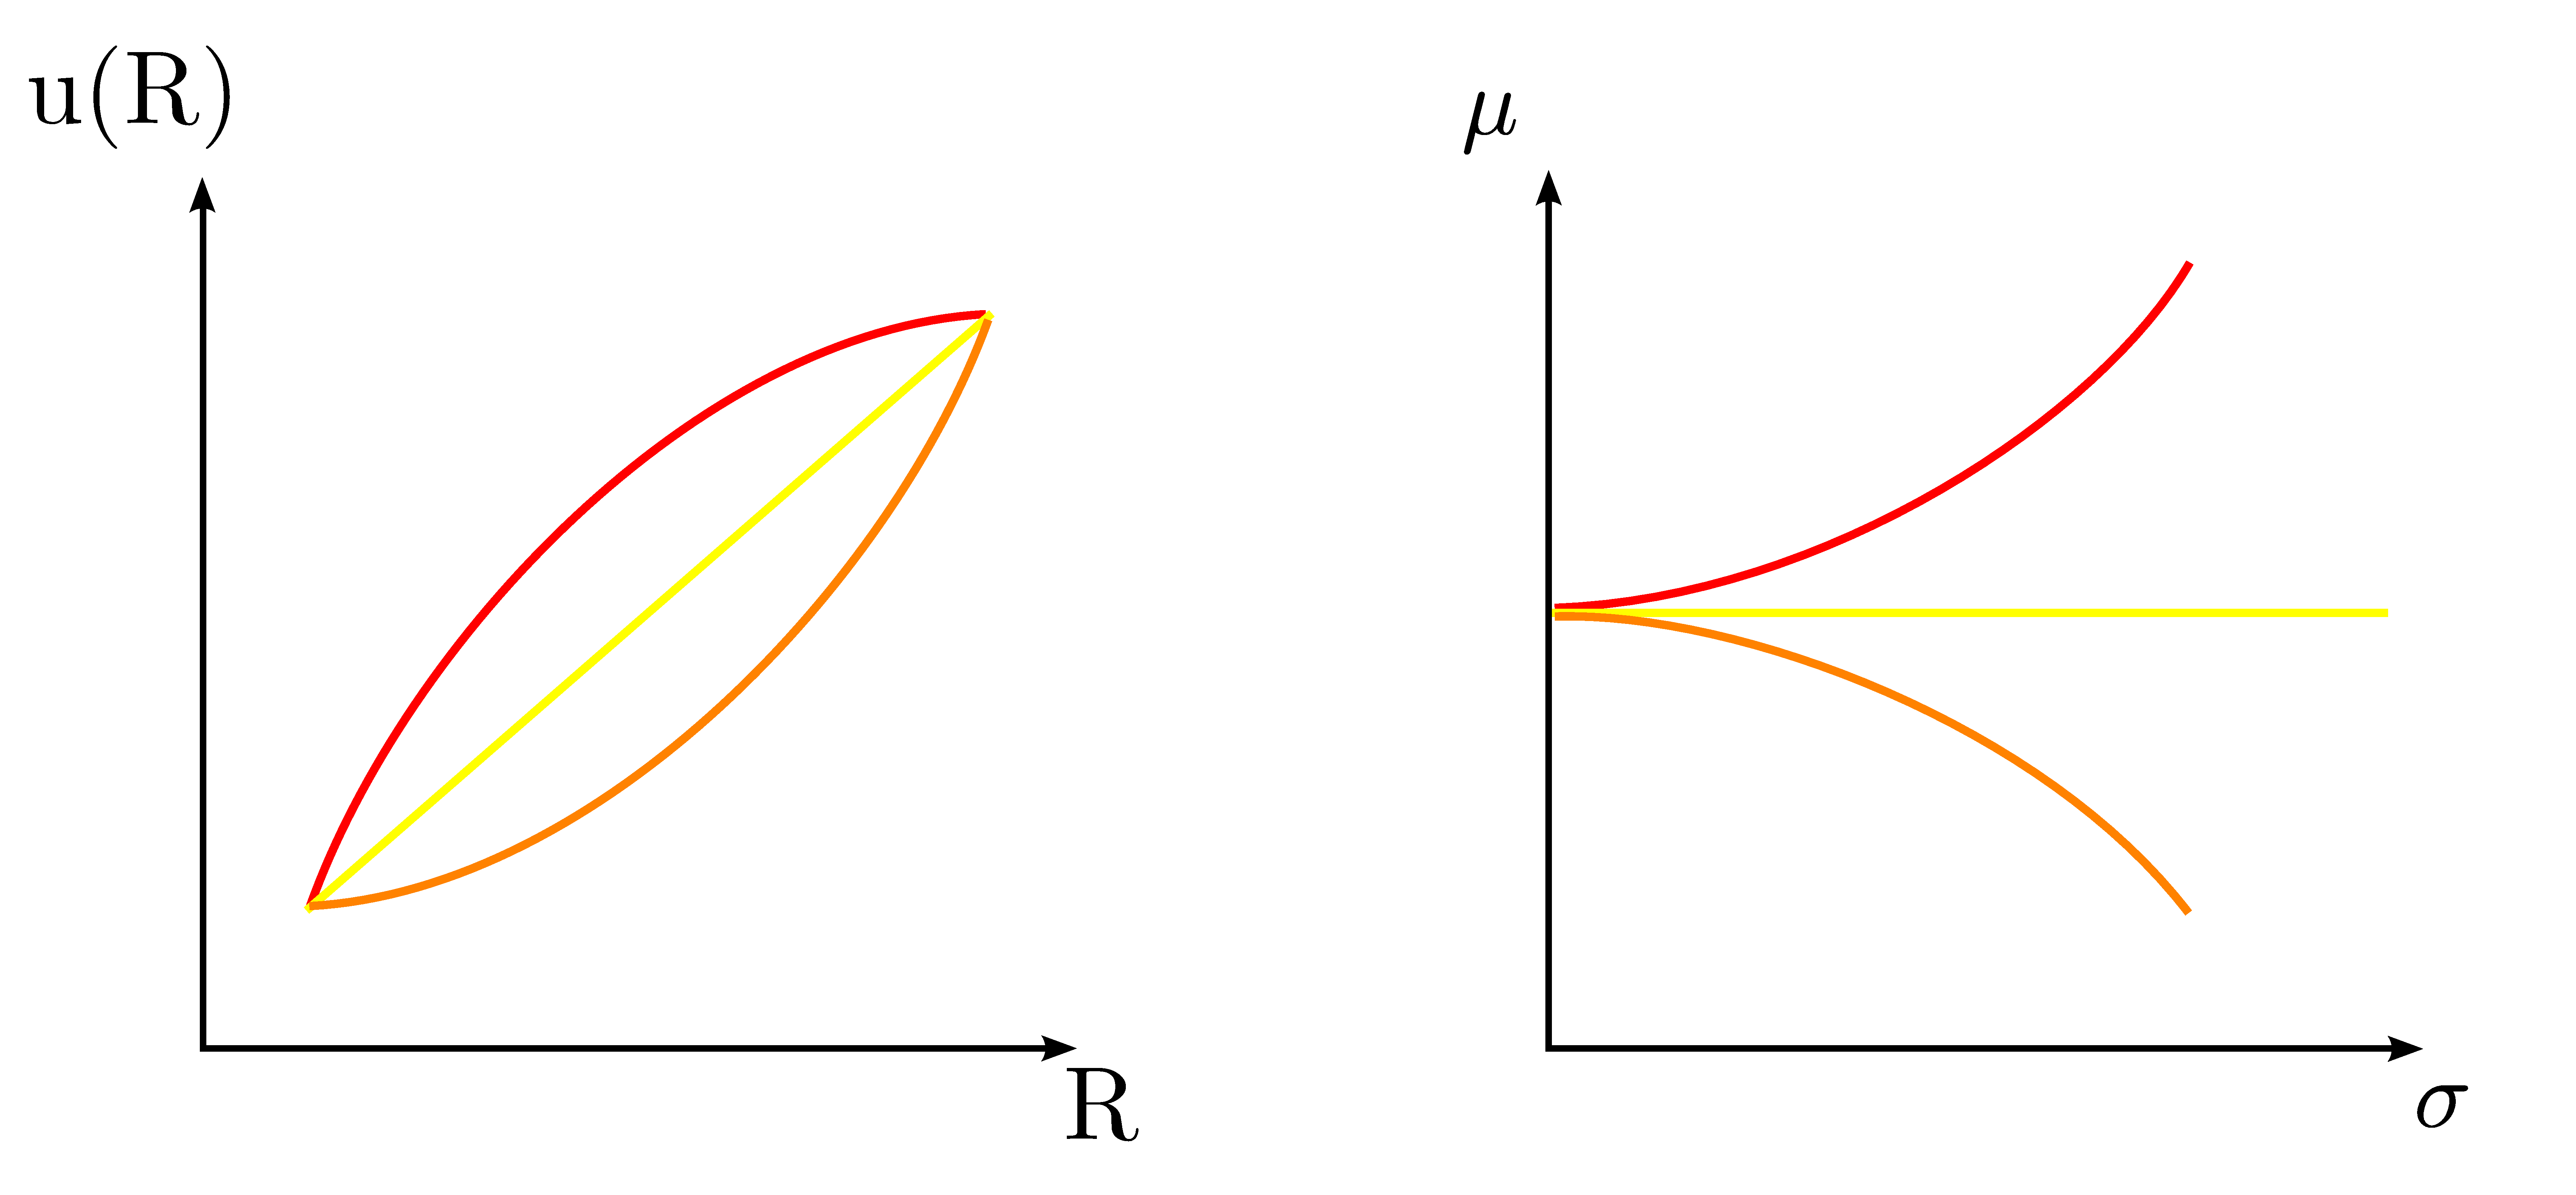
\includegraphics[width=0.8\linewidth]{gfx/risk.pdf}
\caption[Comparison of risk-sensitive behaviors.]{Standard in economic literature, these figures depict the differences between risk-averse (red), risk-neutral (grey) and risk-seeking (orange) behaviors.\\
Left: A subjective utility $u(r)$, based on the reward, is concave for risk-averse behaviors. 
Right: Risk-averse utility contour lines in standard deviation-expected value space are upward sloped.
}
\label{fig:risk}
\end{figure}

The desired behavior for most critical applications is risk-averse and indeed it is the behavior of choice for financial institutions \citep{wipplinger2007philippe, basel2013fundamental}. It has also been suggested that humans use risk-averse behaviors when making decisions \citep{shen2014risk}.

As we stated in the introduction, we are interested in reinforcement learning that maximizes a certain risk-averse objective. Below we formally describe the metrics used to measure risk which we then use to formulate the exact problem tackled in this thesis.

\subsection{Value-at-Risk}

Value-at-risk (VaR, see e.g. \citet{wipplinger2007philippe}) is one of the most popular tools used to estimate exposure to risk used risk management and financial control.

Let $Z$ be a random variable representing reward, with cumulative distribution function (c.d.f.) $F(z) = \mathbb{P}(Z \le z)$.
The Value-at-Risk  at confidence level $\alpha \in (0,1)$ is the $\alpha$-quantile of $Z$, i.e. 
\begin{equation}
\text{VaR}_\alpha(Z)=F^{-1}(\alpha)=\inf\left\lbrace z | \alpha \le F(z) \right\rbrace
\end{equation}

We will use the notation $\text{VaR}_\alpha(Z)$, $F^{-1}(\alpha)$ interchangeably, often explicitly denoting the random variable of inverse c.d.f. as $F^{-1}_Z(\alpha)$.
\\
\\
\textit{Note on notation}: In the risk-related literature, it is common to work with losses instead of rewards. The Value-at-Risk is then defined as the $1-\alpha$ quantile. The notation we use reflects the use of reward in reinforcement learning and this sometimes leads to the need of reformulating some definitions or theorems. While these reformulations may differ in notation, they characterize the same underlying ideas.

\subsection{Conditional Value-at-Risk}

Conditional Value-at-Risk (CVaR, see \citet{rockafellar2000optimization,rockafellar2002conditional}), sometimes called Expected Shortfall (ES), Average Value-at-Risk (AVaR) or Tail Value-at-Risk (TVaR), is a risk measure that aims to fix inadequacies of measuring risk introduced by Value-at-Risk. Firstly, it has the desirable mathematical properties of monotonicity, translation invariance, positive homogeneity and subadditivity (see \citet{artzner1999coherent}), which makes CVaR computation much easier compared to VaR. It's properties were also recently identified as suitable for measuring risk in robotics \cite{majumdar2017should}. Another strong point of CVaR is that unlike VaR, it is able to distinguish between large and catastrophic losses. For these reasons, CVaR is starting to replace VaR as a standard measure for risk in financial applications \citep{basel2013fundamental} and beyond.

The Conditional Value-at-Risk (CVaR) at confidence level $\alpha \in (0,1)$ is defined as the expected reward of of outcomes worse than the $\alpha$-quantile ($\var_\alpha$):
\begin{equation}\label{eqn:cvardef}
\text{CVaR}_\alpha(Z) = \dfrac{1}{\alpha}\int_0^\alpha F^{-1}_Z(\beta) \text{d}\beta = \dfrac{1}{\alpha}\int_0^\alpha \text{VaR}_\beta(Z) \text{d}\beta
\end{equation}
\citet{rockafellar2000optimization} also showed that CVaR is equivalent to the solution of
\begin{equation}\label{eqn:cvarprimal}
\text{CVaR}_\alpha(Z)=
\max_s\left\lbrace \dfrac{1}{\alpha}\expect
\left[ (Z-s)^-\right] + s  \right\rbrace 
\end{equation}
where $(x)^- = \min(x, 0)$ represents the negative part of $x$ and in the optimal point $s^* = VaR_\alpha(Z)$
\begin{equation}
\text{CVaR}_\alpha(Z)= \dfrac{1}{\alpha}\expect \left[ (Z-VaR_\alpha(Z))^-\right] + VaR_\alpha(Z)
\end{equation}

The last definition we will need is the dual formulation of \eqnref{cvarprimal}
\newcommand{\smallenvelope}{\mathcal{U}_{\cvar}(\alpha, p(\cdot))}
\begin{align}\label{eqn:cvardual}
&\cvar_\alpha(Z)= \min_{\xi \in \smallenvelope}\expect\nolimits_\xi[Z]\\
&\smallenvelope = \braces{\xi : \xi(z) \in \bsquare{0, \frac{1}{\alpha}}, \int \xi(z)p(z) \text{d}z = 1}\label{eqn:envelope}
\end{align}
We provide basic intuition behind the dual variables as these will become important later: Since we are minimizing the variables $\xi$ over the set $\smallenvelope$, the optimal values are $\xi(z) = \min\left(\frac{1}{\alpha}, \frac{1}{p(z)}\right)$ for the lowest possible values $z$, as these 
values influence the resulting $\cvar_\alpha(Z)$. Values above $\var_\alpha(Z)$ are not taken into account so their $\xi$ is $0$. If there exists a discrete atom at $\var_\alpha(Z)$, the variables are linearly interpolated to fit the constraints.

For a concise treatment of duality, see e.g. \citet{boyd2004convex}.


\begin{figure}
\center
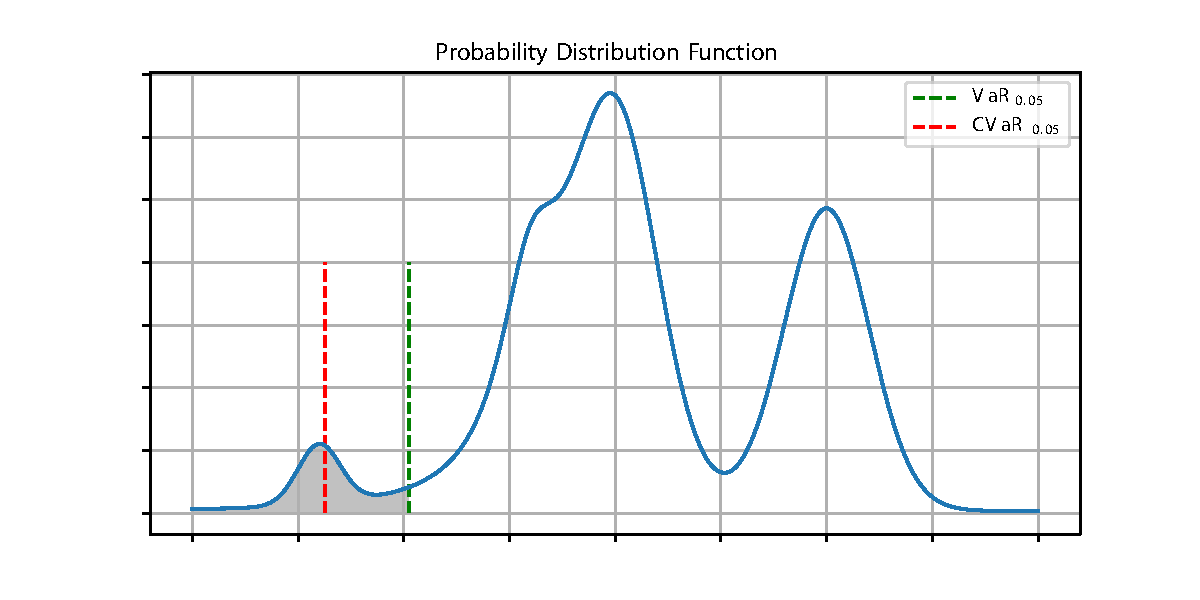
\includegraphics[width=\linewidth]{gfx/pdf.pdf}
\caption[VaR and CVaR of a general probability distribution.]{Value-at-Risk and Conditional Value-at-Risk of a general probability distribution with the integral $\alpha=0.05$ marked in grey. The main flaw of the VaR metric is clearly visible here, as we could shift the leftmost 'mode' of the distribution into minus infinity and the VaR would remain unchanged, while CVaR would change with the shift.}
\end{figure}




%*****************************************
%*****************************************
%*****************************************

\section{Problem Formulation}\label{sec:prelim:problem}

The problem tackled in this thesis considers reinforcement learning with optimization of the CVaR objective. Unlike the expected value criterion, it is insufficient to consider only stationary policies, and we must work with general history-dependent policies. We define them formally below.

\begin{definition}[History-Dependent Policies]
Let the space of admissible histories up to time $t$ be $H_t = H_{t-1} \times \cA \times \cX$ for $t \ge 1$, and $H_0 = \cX$. A generic element $h_t \in H_t$ is of the form $h_t = (x_0, a_0, ..., x_{t-1}, a_{t-1})$. Let $\Pi_{H,t}$ be the set of all history-dependent policies with the property that at each time $t$ the randomized control action is a function of $h_t$. In other words, 
$\Pi_{H,t} = \braces{\pi_0: H_0 \to \mathbb{P}(\cA), ..., \pi_t: H_t \to \mathbb{P}(\cA)}$. We also let $\Pi_H = \lim_{t\to\infty}\Pi_{H,t}$ be the set of all history-dependent policies.
\end{definition}

The risk-averse objective we wish to address for a given confidence level $\alpha$ is
\begin{equation}\label{eqn:problem}
\max_{\pi \in \Pi_H} \text{CVaR}_\alpha(Z^\pi(x_0))
\end{equation}
where $Z^\pi(x_0)$ coincides with definition \eqnref{return}.

In words, our goal is to find a general policy $\pi^*\in \Pi_H$, that maximizes conditional value-at-risk of the return, starting in state $x_0$. We emphasize the importance of the starting state since, unlike the expected value, the CVaR objective is not time-consistent.


\subsection{Time-consistency}\label{sec:time}

There exist several definitions of time-consistency \citep{pflug2016time, boda2006time}.
Informally, if the criterion is time-consistent, we can limit ourselves to the space of stationary policies, as the optimal policy is part of this space. On the other hand, non-stationary policies may be required to solve a time-inconsistent problem.

We provide the following example to show that the CVaR criterion is indeed time-inconsistent. In \figref{time-consistency} we can see an MDP with starting state $x_1$ with a single action $a_0$, followed by state $x_2$ where the agent can choose between actions $a_1, a_2$; states $x_3, x_4$ are terminal. We now compare three policies $\pi_1(x_1)=a_1, \pi_2(x_1)=a_2$ and a non-stationary policy $\pi_3$ that chooses $a_2$, unless the agent was lucky and received the reward 10 when transitioning from state $x_1$.
Let us examine the CVaR objective with $\alpha=0.19$ and $\gamma=1$ (or close to 1):
\begin{align*}
&\cvar_{0.19}(Z^{\pi_1}(x_1))=\frac{0.19 \cdot 0}{0.19} = 0\\
&\cvar_{0.19}(Z^{\pi_2}(x_1))=\frac{0.09\cdot (-10) + 0.01 \cdot 0 + 0.09 \cdot 10}{0.19}=0\\
&\cvar_{0.19}(Z^{\pi_3}(x_1))=\frac{0.09 \cdot (-10)+ 0.1 \cdot 10}{0.19} \cca 0.526
\end{align*}
By examining the results, we can see that the non-stationary policy $\pi_3$ is better than any stationary one, confirming CVaR as a time-inconsistent objective, explaining the need for a history-dependent policy in our problem definition \ref{eqn:problem}.

As we will see later, the time-inconsistency can be sidestepped by extending the state space by a continuous parameter $y \in [0, 1]$ which represents the different confidence levels we may choose to optimize. Notably, the optimal policy must in this case consider different confidence levels in each state - otherwise we would consider only stationary policies.

\begin{figure}
\center
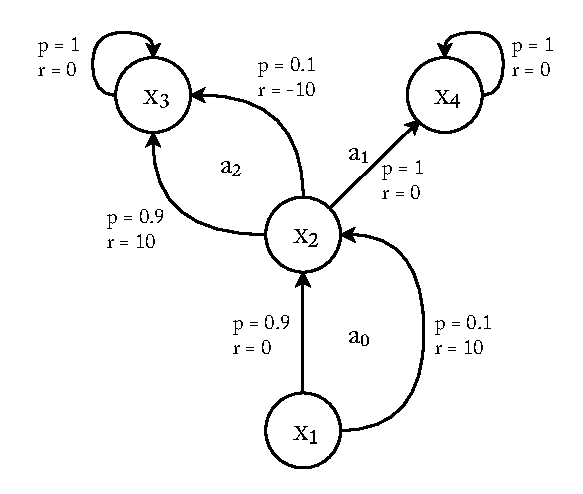
\includegraphics[width=0.6\linewidth]{gfx/time.pdf}
\caption{MDP showing time-inconsistency of the CVaR objective.}
\label{fig:time-consistency}
\end{figure}

\subsection{Robustness}

An important motivational point for the CVaR objective \eqnref{problem} is it's relationship with robustness. \citet{chow2015risk} have shown that optimizing the objective is equivalent to being robust to model perturbations. Thus, by minimizing CVaR, the decision maker also guarantees robustness to modeling errors. For completeness, we repeat the formulation of the equivalence relation below.

Let $(x_0, a_0, ..., x_T)$ be a trajectory in a finite-horizon MDP problem. The total probability of the trajectory is $p(x_0, a_0, ..., x_T)=p(x_0)p(x_1|x_0,a_0)\cdots p(x_T|x_{T-1}, a_{T-1})$. For each step $1\le t\le T$ consider a perturbed transition matrix $\hat{P} = P \circ \delta_t$ where $\delta_t \in \real^{\cX\times\cA\times\cX}$ and $\circ$ is the element-wise product under the condition that $\hat{P}$ is a stochastic matrix. Let $\Delta_t$ be the set of perturbation matrices that satisfy this condition and $\Delta = \Delta_1 \times \cdots \times \Delta_T$ be the set of all possible perturbations to the trajectory distribution.

We now impose a budget constraint on the perturbations as follows. For some budget $\eta \geq 1$, we consider the constraint
\begin{equation}\label{eqn:budget}
    \delta_1(x_1|x_0)\delta_2(x_2|x_1)\cdots \delta_T(x_T|x_{T-1}) \leq \eta
\end{equation}
Essentially, the product in \eqref{eqn:budget} states that \emph{the worst cannot happen at each time}. Instead, the perturbation budget has to be split (multiplicatively) along the trajectory. We note that \eqref{eqn:budget} is in fact a constraint on the perturbation matrices, and we denote by $\Delta_\eta \subset \Delta$ the set of perturbations that satisfy this constraint with budget $\eta$.
Then the following holds (Proposition 1 of \citep{chow2015risk})
\begin{equation}\label{eq:CVaR_is_robustness}
    \text{CVaR}_{\frac{1}{\eta}} \left(R_{0,T}(x_1,\dots,x_T)\right) = \inf_{(\delta_1,\dots,\delta_T)\in \Delta_{\eta}} \expect\nolimits_{\hat{P}}[R_{0,T}(x_1,\dots,x_T)],
\end{equation}
where $R_{0,T}(x_1,\dots,x_T)$ denotes the random variable representing the reward along the particular trajectory and $\expect\nolimits_{\hat{P}}[\cdot]$ denotes expectation with respect to a Markov chain with transitions $\hat{P}_t$.


%*****************************************
%*****************************************
%*****************************************



\section{Literature Survey}\label{sec:prelim:literature}

Risk-sensitive MDPs have been studied thoroughly in the past, with different risk-related objectives. Due to it's good computational properties, earlier efforts focused on exponential utility \citep{howard1972risk}, the max-min criterion \citep{coraluppi1998optimal} or e.g. maximizing the mean with constrained variance \citep{sobel1982variance}. A comprehensive overview of the different objectives can be found in \citet{garcia2015comprehensive}, together with a unified look on the different methods used in safe reinforcement learning. Among CVaR-related objectives, some publications focus on optimizing the expected value with a CVaR constraint \citep{borkar2010risk, prashanth2014policy}.

Recently, for the reasons explained above, several authors have investigated the exact objective \eqnref{problem}. A considerable effort has gone towards policy-gradient \citep{sutton2000policy} and Actor-Critic \citep{konda2000actor} algorithms with the CVaR objective. \citet{tamar2015optimizing, chow2014algorithms} present useful ways of computing the CVaR gradients with parametric models and have shown the practicality and scalability of these approaches on interesting domains such as the well-known game of Tetris. An important setback of these methods is their limitation of the hypothesis space to the class of stationary policies, meaning they can only reach a $local$ minimum of our objective.
Similar policy gradient methods have also been investigated in the context of general coherent measures, a class of risk measures encapsulating many used measures including CVaR. Tamar et al. present a policy gradient algorithm and a gradient-based Actor-Critic algorithm \citep{tamar2017sequential}. Again, these algorithms only converge in local extremes.

Some authors have also tried to sidestep the time-consistency issue of CVaR by either focusing on a time-consistent subclass of coherent measures, limiting the hypothesis space to time-consistent policies, or reformulating the CVaR objective in a time-consistent way \cite{miller2017optimal}.

\citet{morimura2010nonparametric, morimura2012parametric} were among the first to utilize distributional reinforcement learning with both parametric and nonparametric models and used it to optimize CVaR. They only used the naive approach discussed in \secref{time} in their experiments.

\citet{bauerle2011markov} use a state space extensions and show that this new extended state space contains globally optimal policies. Unfortunately, because the state-space is continuous, the design of a solution algorithm is challenging.

The approach of \citet{chow2015risk} also uses a continuous augmented state-space but unlike \citet{bauerle2011markov}, this continuous state is shown to have bounded error when a particular linear discretization is used. The only flaw of this approach is the requirement of running a linear program in each step of their algorithm and we address this issue in the next chapter.


%Risk-sensitive MDPs have been studied for over four decades, with earlier efforts focusing on exponential utility \cite{Howard1972Risk}, mean-variance \cite{sobel_variance_1982}, and percentile risk criteria \cite{filar_percentile_1995} . Recently, for the reasons explained above, several authors have investigated CVaR MDPs \cite{rockafellar2000optimization}. Specifically, in \cite{borkar2014risk}, the authors propose a dynamic programming algorithm for finite-horizon risk-constrained MDPs where risk is measured according to CVaR. The algorithm is proven to asymptotically converge to an optimal risk-constrained policy. However, the algorithm involves computing  integrals over continuous variables (Algorithm 1 in \cite{borkar2014risk}) and, in general, its implementation appears particularly difficult. In \cite{bauerle2011markov}, the authors investigate the structure of CVaR optimal policies and show that a Markov policy is optimal on an augmented state space, where the additional (continuous) state variable is represented  by the running cost. In \cite{haskell2014convex}, the authors leverage such result to design an algorithm for CVaR MDPs that relies on discretizing occupation measures in the augmented-state MDP. This approach, however, involves solving a non-convex program via a sequence of linear-programming approximations, which can only shown to converge asymptotically. A different approach is taken by \cite{chow2014cvar} and \cite{tamar2015optimizing}, which consider a finite dimensional parameterization of control policies, and show that a CVaR MDP can be optimized to a \emph{local} optimum using stochastic gradient descent (policy gradient). A recent result by Pflug and Pichler \cite{pflug2012time} showed that CVaR MDPs admit a dynamic programming formulation by using a state-augmentation procedure different from the one in \cite{bauerle2011markov}. The augmented state  is also continuous, making the design of a solution algorithm challenging. 

%\subsection{Safe Reinforcement Learning}
%
%\citep{garcia2015comprehensive}
%\citep{bauerle2011markov}
%
%
%
%
%\subsection{Reinforcement Learning with CVaR-related criteria}
%
%*** Policy gradient literature ignores the time consistency-issue, leading to locally optimal policies show that they can be worse than EXP ***.
%\citep{tamar2015policy}
%\citep{tamar2015optimizing}
%\citep{chow2014algorithms}

